\section{Numerical verification and validation}
\subsection{Manufactured solution for the immersed Vlasov equation}

We first verify the advection part of the solver in the absence of external forces.
The governing equation reduces to a pure 2D2V advection problem:
\begin{equation}
\frac{\partial f}{\partial t}
+ v_x \frac{\partial f}{\partial x}
+ v_y \frac{\partial f}{\partial y}
= 0,
\end{equation}
where \(f = f(x,y,v_x,v_y,t)\) is the distribution function.

The physical domain is \([0,1] \times [0,0.5]\) and the velocity domain is \([-0.05, 0.95] \times [-0.5, 0.5]\).  
Periodic boundary conditions are imposed in all phase‑space directions.  
An absorbing cylinder is defined by the level‑set function
\(\eta(x,y) = (x-0.375)^2 + y^2 - 0.125^2\); on this immersed boundary the distribution function is set to zero.

The initial condition is a Gaussian pulse in \(x\) and a Dirac delta in velocity,
\begin{equation}
f(x,y,v_x,v_y,0) =
\frac{1}{\Delta v_x \Delta v_y}\,
\exp\!\left(-\left(\frac{x - x_0}{0.05}\right)^{\!2}\right)
\delta(v_x-C,\, v_y),
\end{equation}
where \(\delta\) denotes the two‑dimensional Dirac delta, \(C\) is a constant drift velocity, and \(\Delta v_x,\Delta v_y\) are the velocity grid spacings (the factor \(1/(\Delta v_x\Delta v_y)\) approximates the delta in the discrete setting).  
Thus, the particles move with constant velocity in the \(x\) direction, and the Poisson equation is disabled.

This configuration benchmarks the ability of the scheme to capture advection, interaction with an immersed boundary, and particle loss due to absorption as the pulse propagates across the domain and encounters the cylinder.  
The convergence study (Fig.~\ref{fig:advection_convergence}) shows that the solver recovers third‑order accuracy in free space and second‑order accuracy near the immersed boundary.

\begin{figure}[htbp!]
	\centering
	\subfloat[Number density]{
		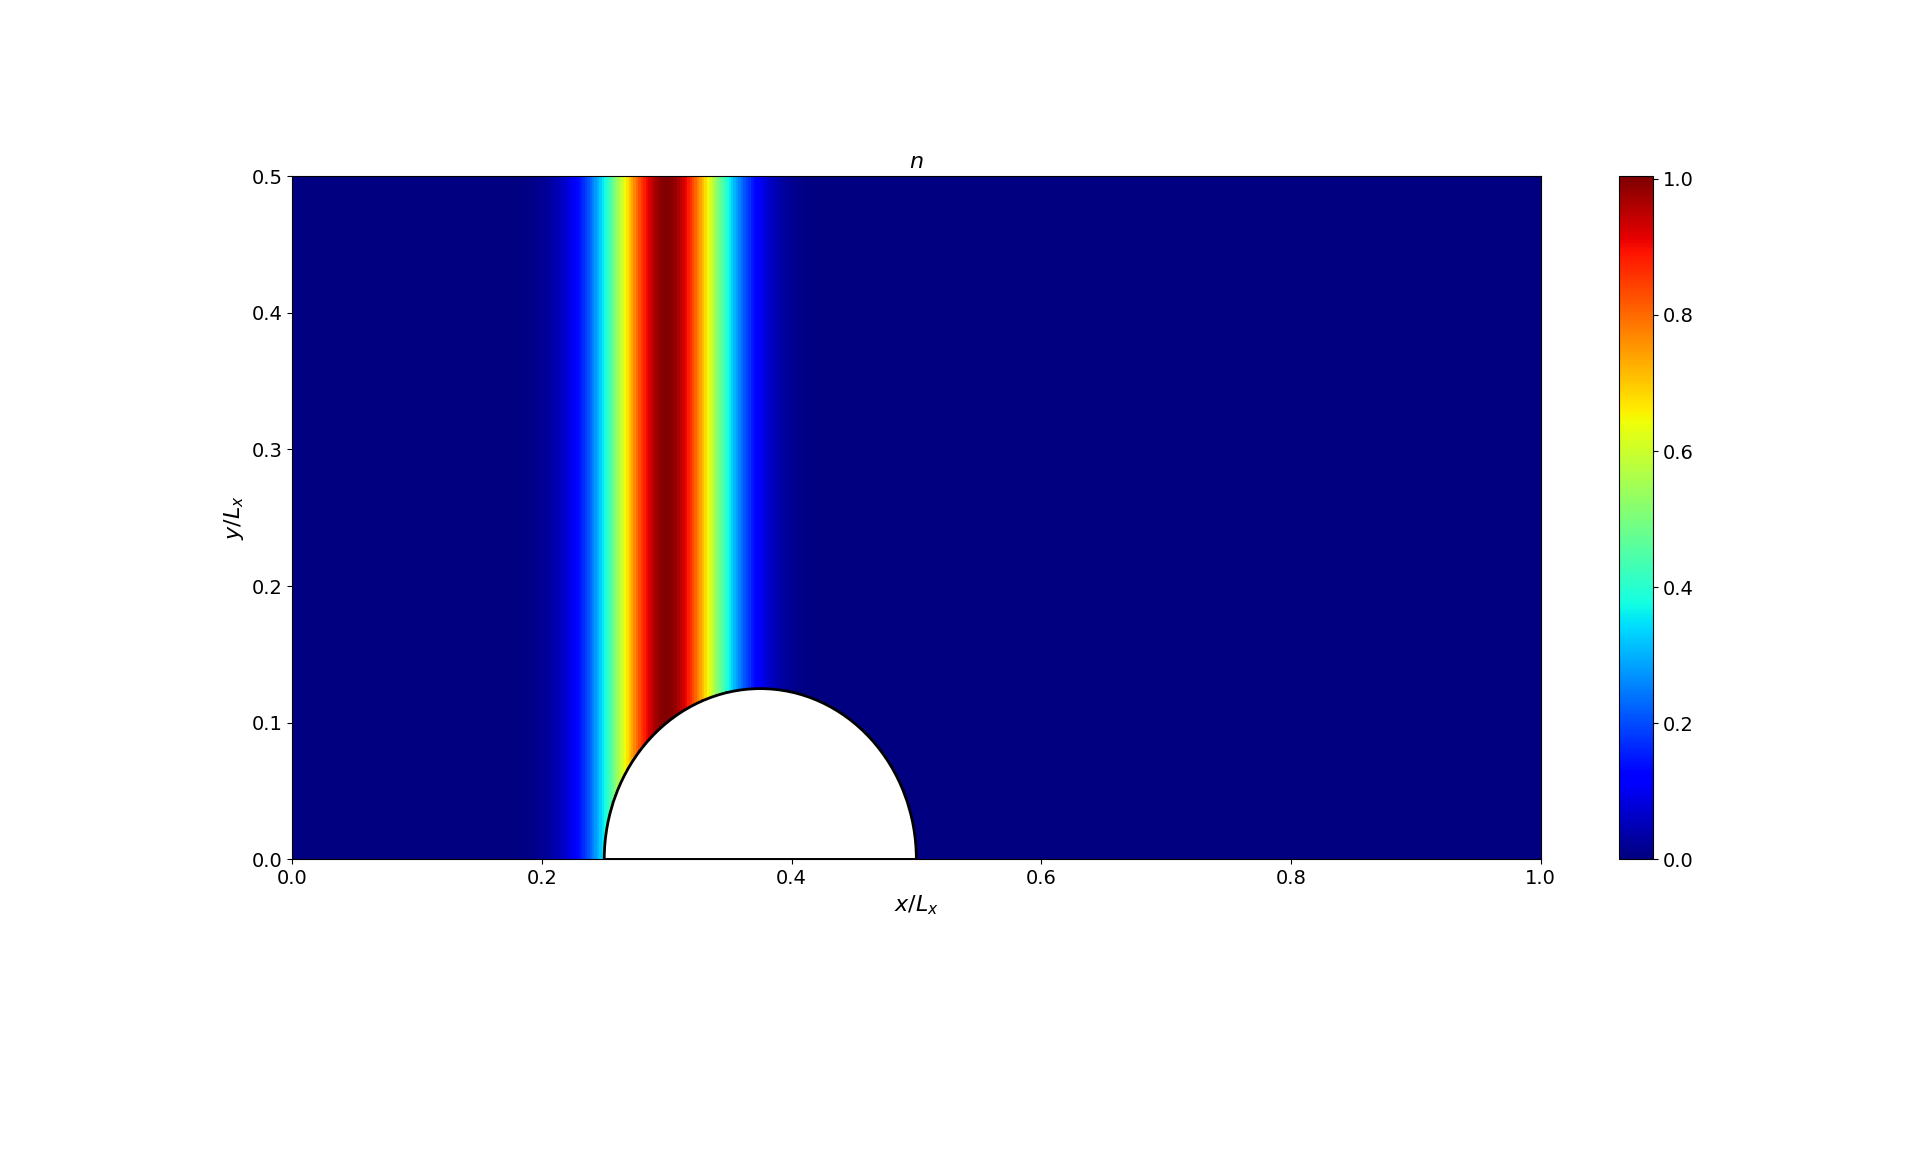
\includegraphics[width=0.5\textwidth]{figures/advection_number_density.png}
	}
	\subfloat[Number density profiles]{
		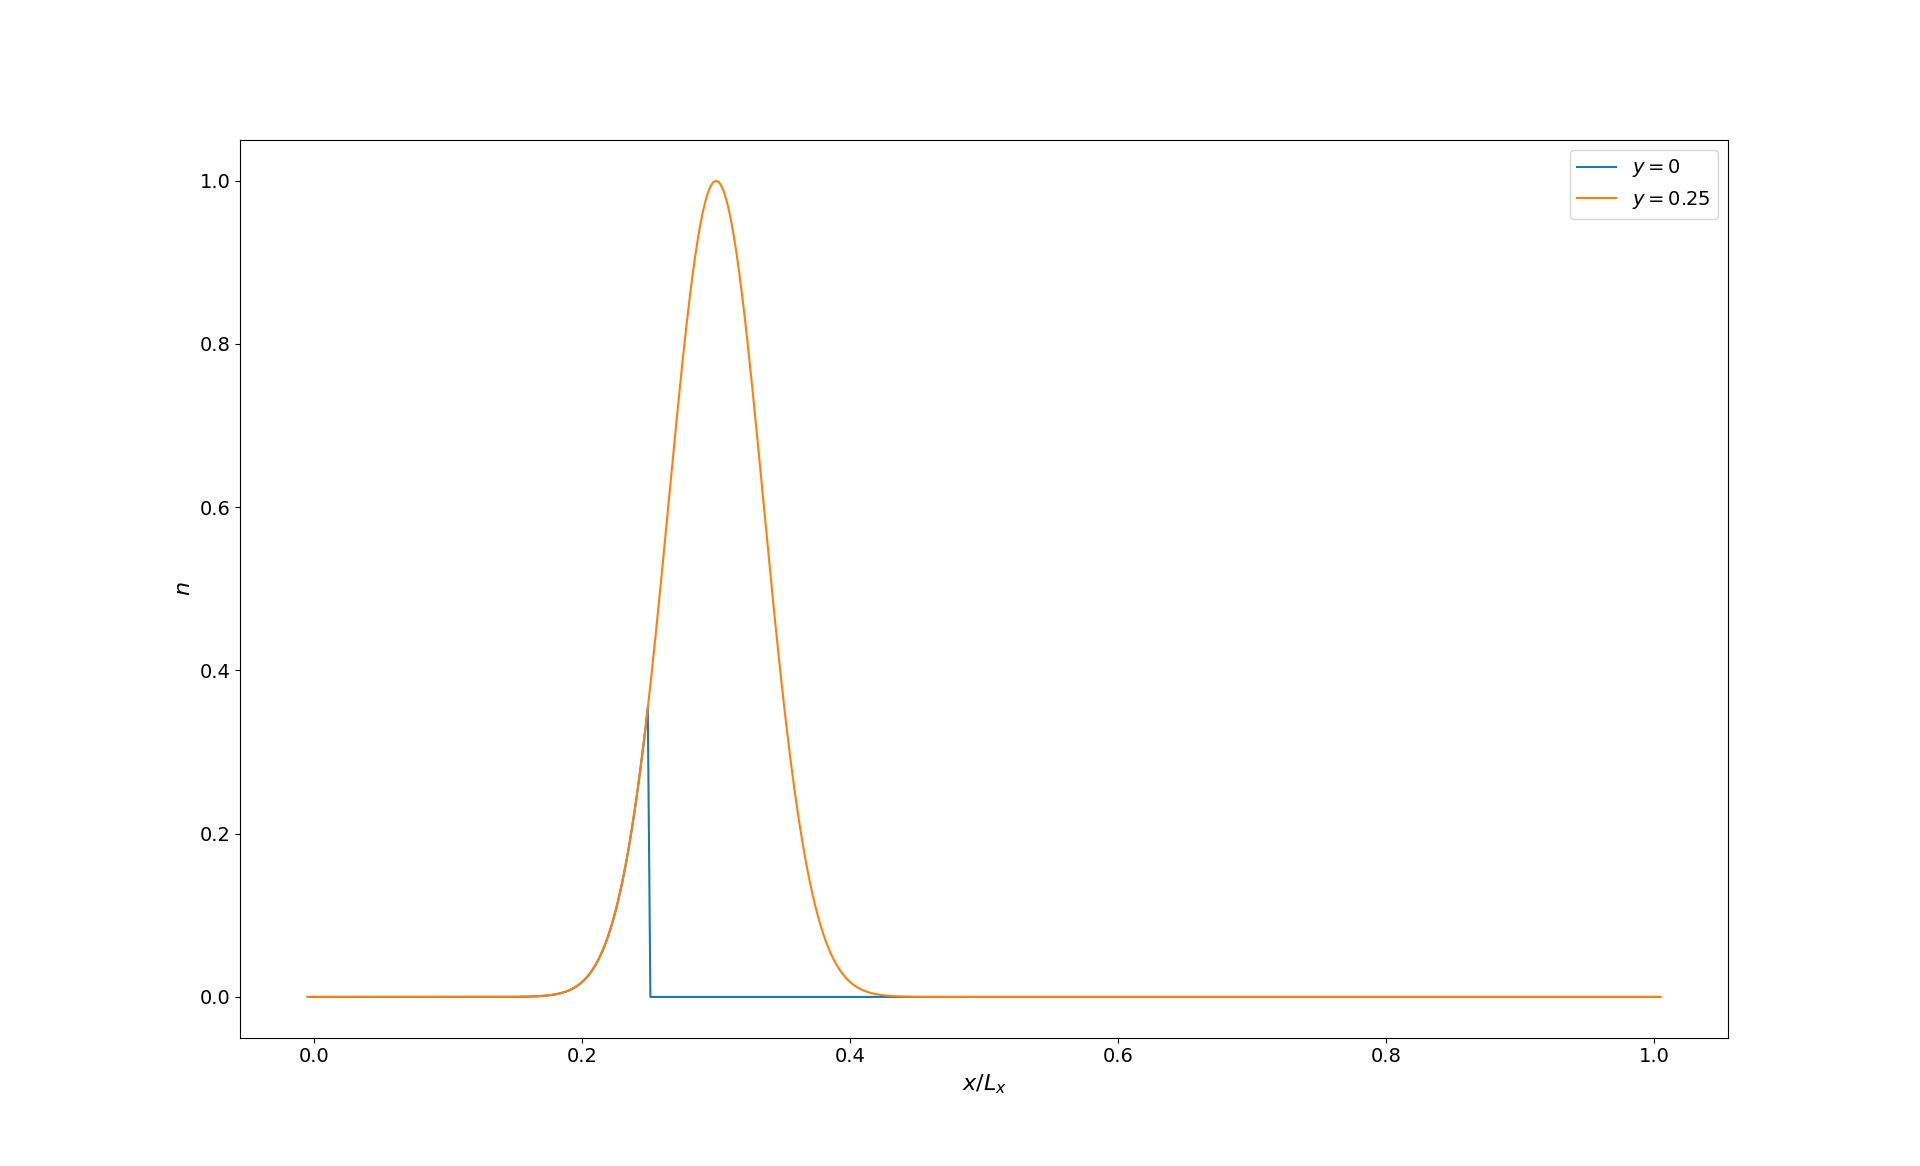
\includegraphics[width=0.5\textwidth]{figures/advection_number_density_profiles.png}
	}
	\label{fig:advection}
\end{figure}

\begin{figure}[htbp!]
	\centering
	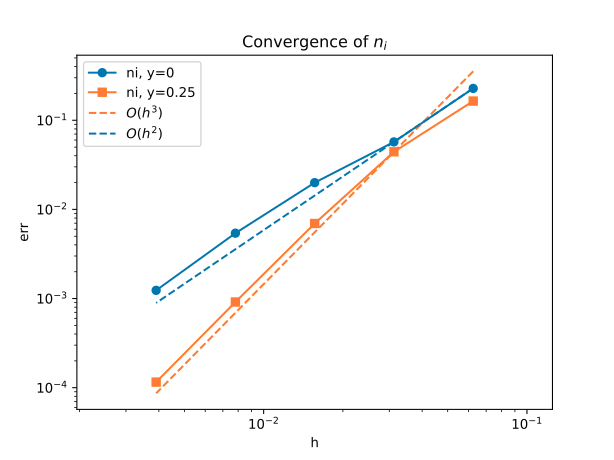
\includegraphics[width=\textwidth]{figures/convergence_advection.png}
	\caption{Convergence study: second‑order accuracy is achieved near the immersed boundary.}
	\label{fig:advection_convergence}
\end{figure}


\subsection{Manufactured solution for the Poisson equation}

Having verified the advection solver, we now turn off the advection and examine the accuracy and convergence order of the Poisson solver in isolation.

The computational domain is \(\Omega = [0,1] \times [0,1]\) with homogeneous Dirichlet conditions on the outer boundary.  
An immersed circular interface \(\Gamma\) is introduced via the level‑set function
\(\eta(x,y) = (x - 0.5)^2 + (y - 0.5)^2 - 0.25^2\).  
The permittivity \(\epsilon\) jumps across \(\Gamma\):
\begin{equation}
\epsilon(x,y) =
\begin{cases}
2, & (x,y) \in \Omega^{-}, \\
1, & (x,y) \in \Omega^{+},
\end{cases}
\end{equation}
where \(\Omega^{-}\) is the interior of the circle and \(\Omega^{+}\) the exterior.  
A charge density is defined only inside the immersed region:
\begin{equation}
\rho(x,y) =
\begin{cases}
-8\,(x^2 + y^2 - 1)\,\exp\big(-(x^2 + y^2)\big), & (x,y) \in \Omega^{-}, \\
0, & (x,y) \in \Omega^{+}.
\end{cases}
\end{equation}

To test the accuracy of the Poisson solver with jump conditions, we prescribe the potential jump and the surface charge density on \(\Gamma\):
\begin{align}
[\phi]_\Gamma &= -\exp\big(-(x^2 + y^2)\big), \\
\left[ \epsilon \frac{\partial \phi}{\partial n} \right]_\Gamma
&=
8\,(2x^2 + 2y^2 - x - y)\,
\exp\big(-(x^2 + y^2)\big).
\end{align}

The convergence study (Fig.~\ref{fig:poisson_convergence}) demonstrates that the solver attains second‑order accuracy even in the presence of these jumps.

\begin{figure}[htbp!]
	\centering
	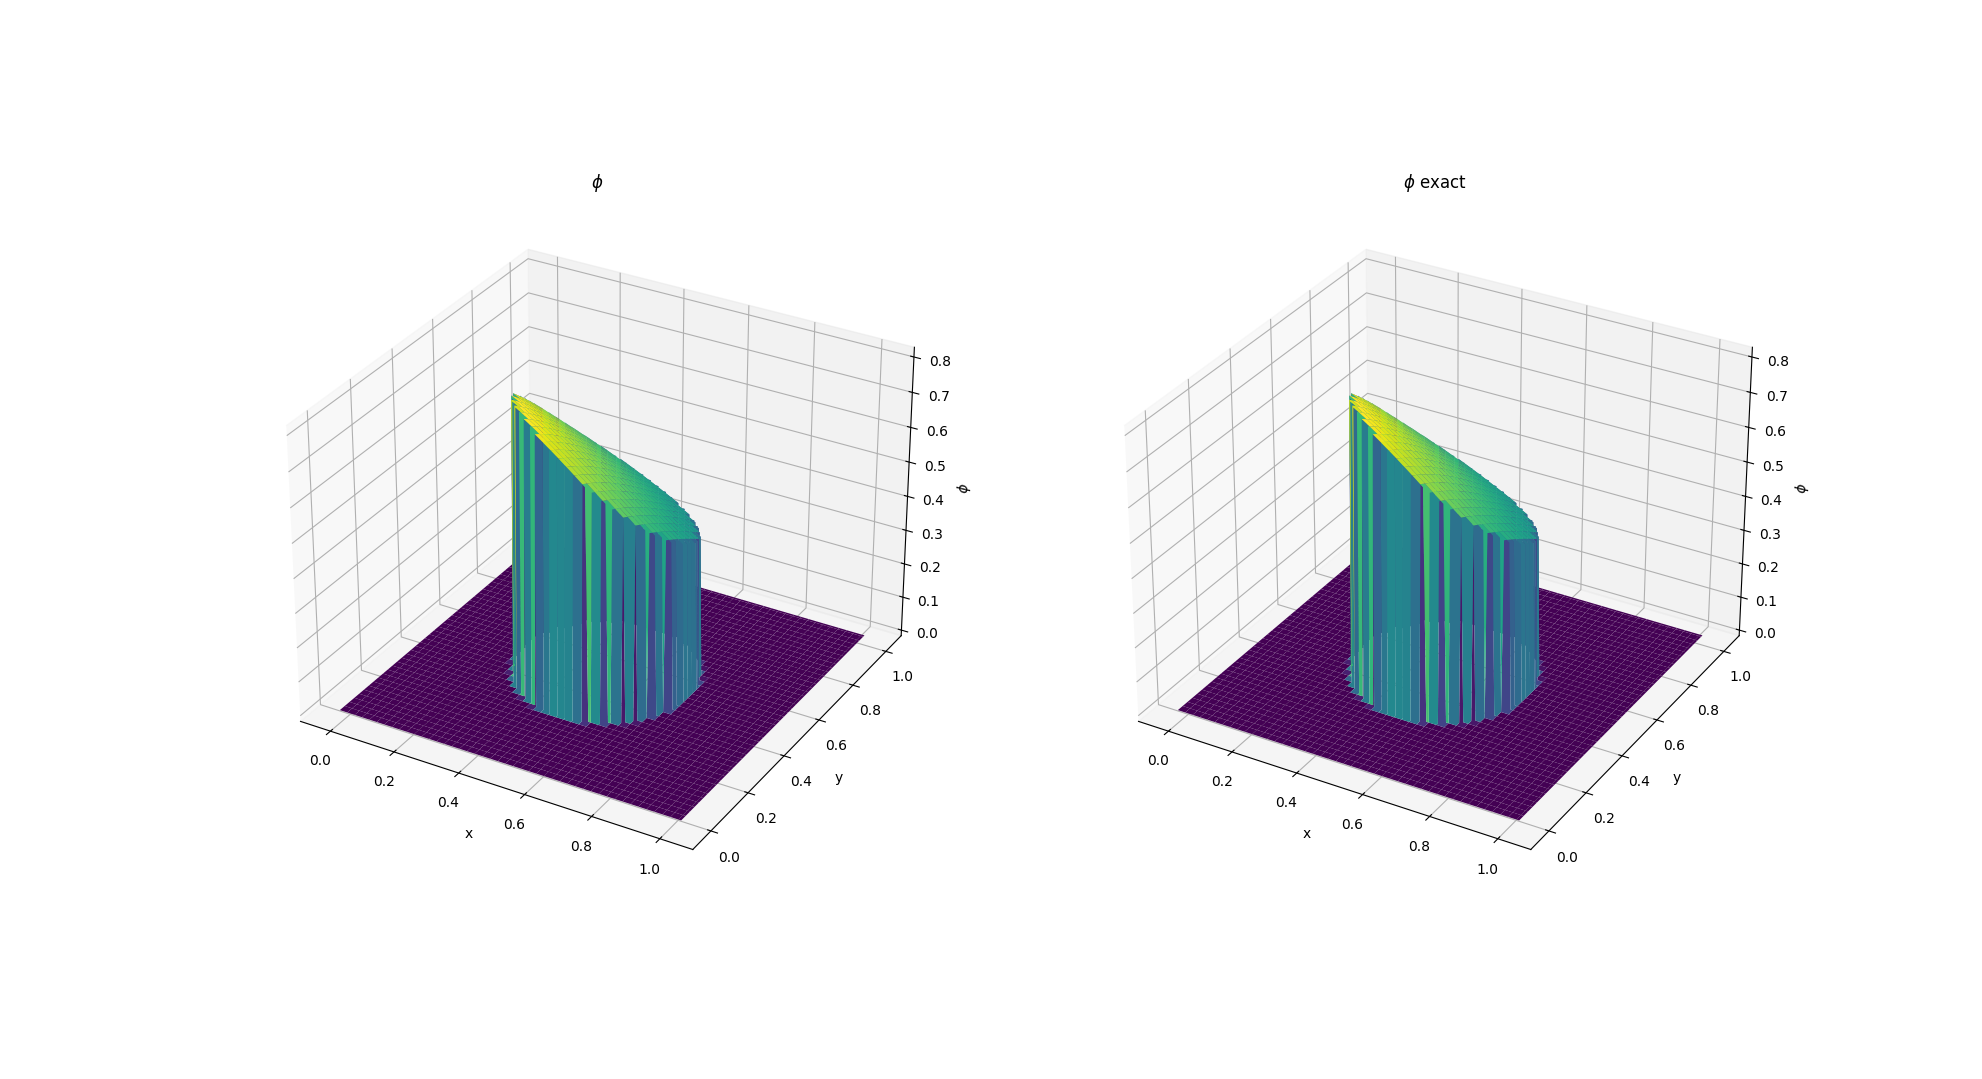
\includegraphics[width=\textwidth]{figures/poisson_solution.png}
	\caption{Numerical solution of the Poisson equation for the manufactured problem.}
	\label{fig:poisson_solution}
\end{figure}

\begin{figure}[htbp!]
	\centering
	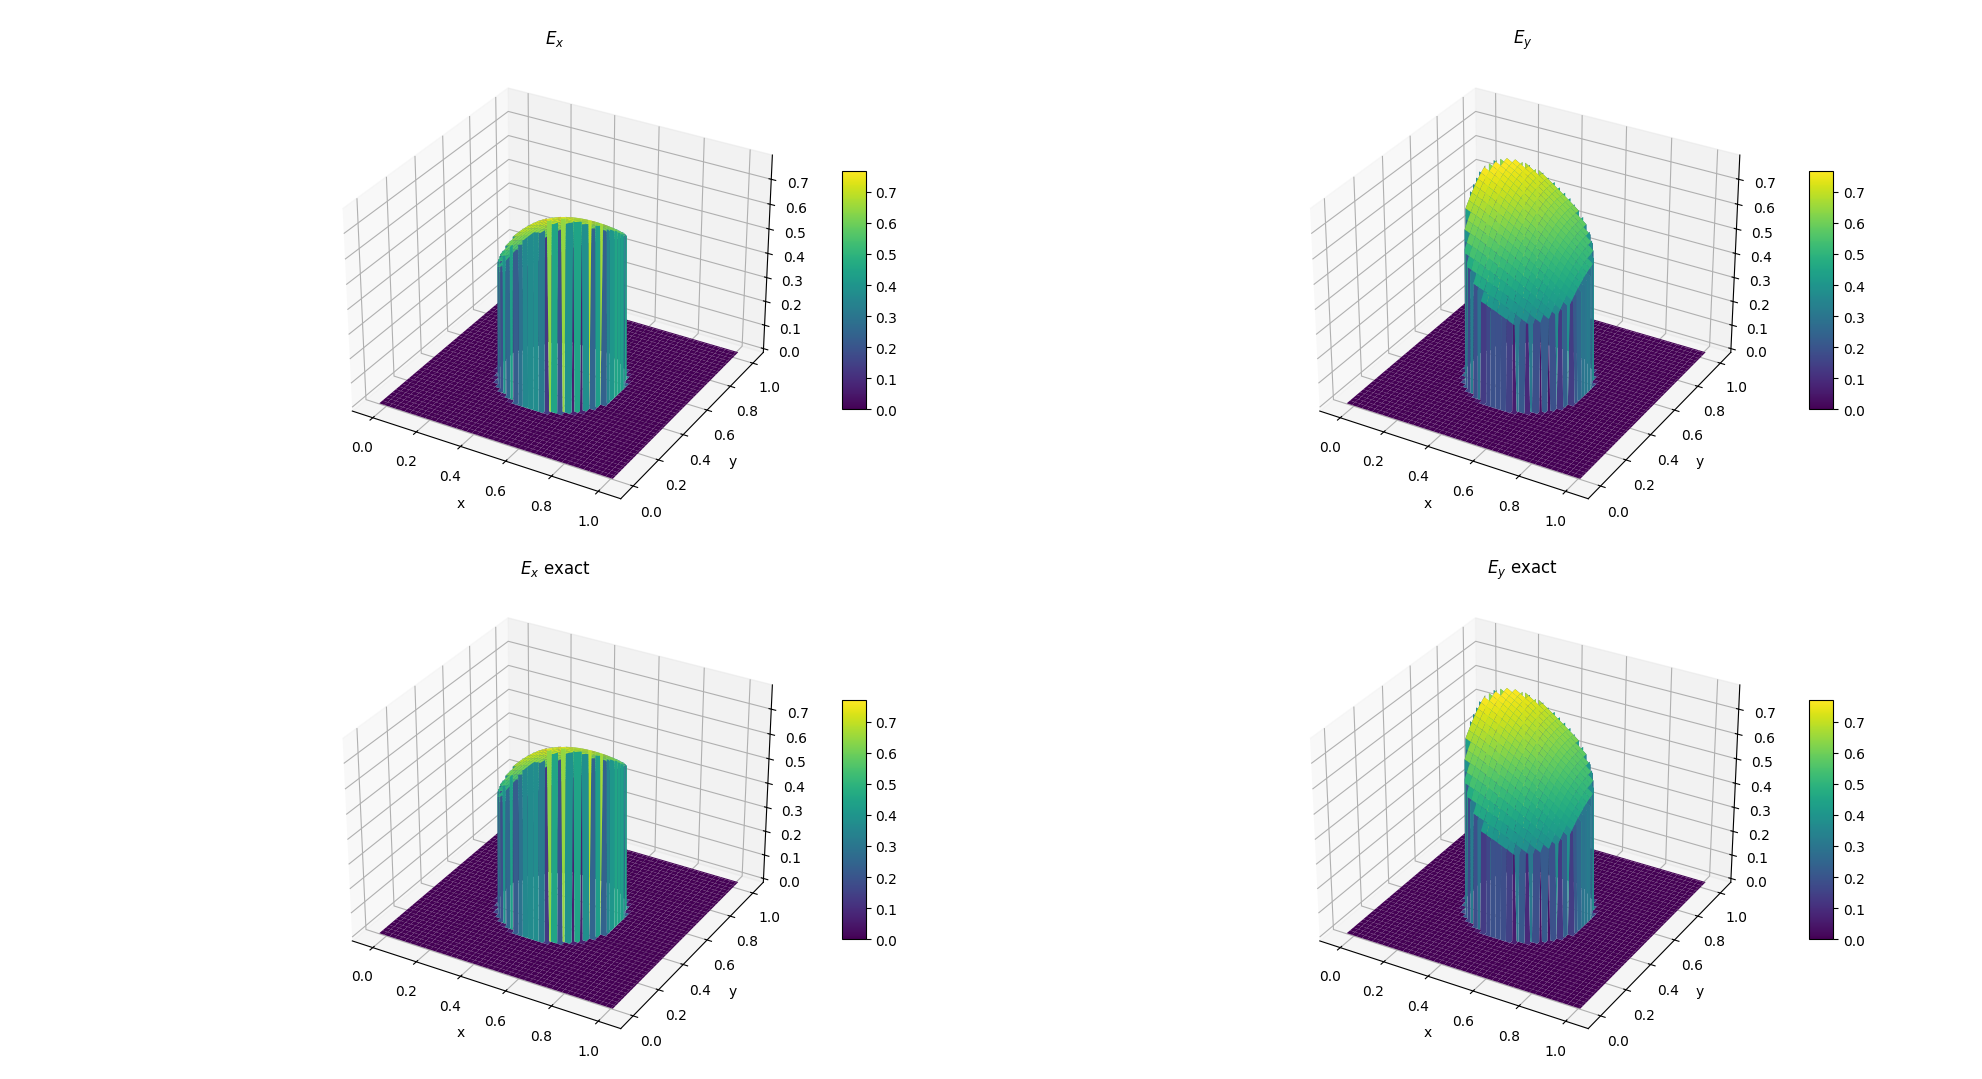
\includegraphics[width=\textwidth]{figures/poisson_gradient.png}
	\caption{Negative gradient of the numerical potential.}
	\label{fig:poisson_gradient}
\end{figure}

\begin{figure}[htbp!]
	\centering
	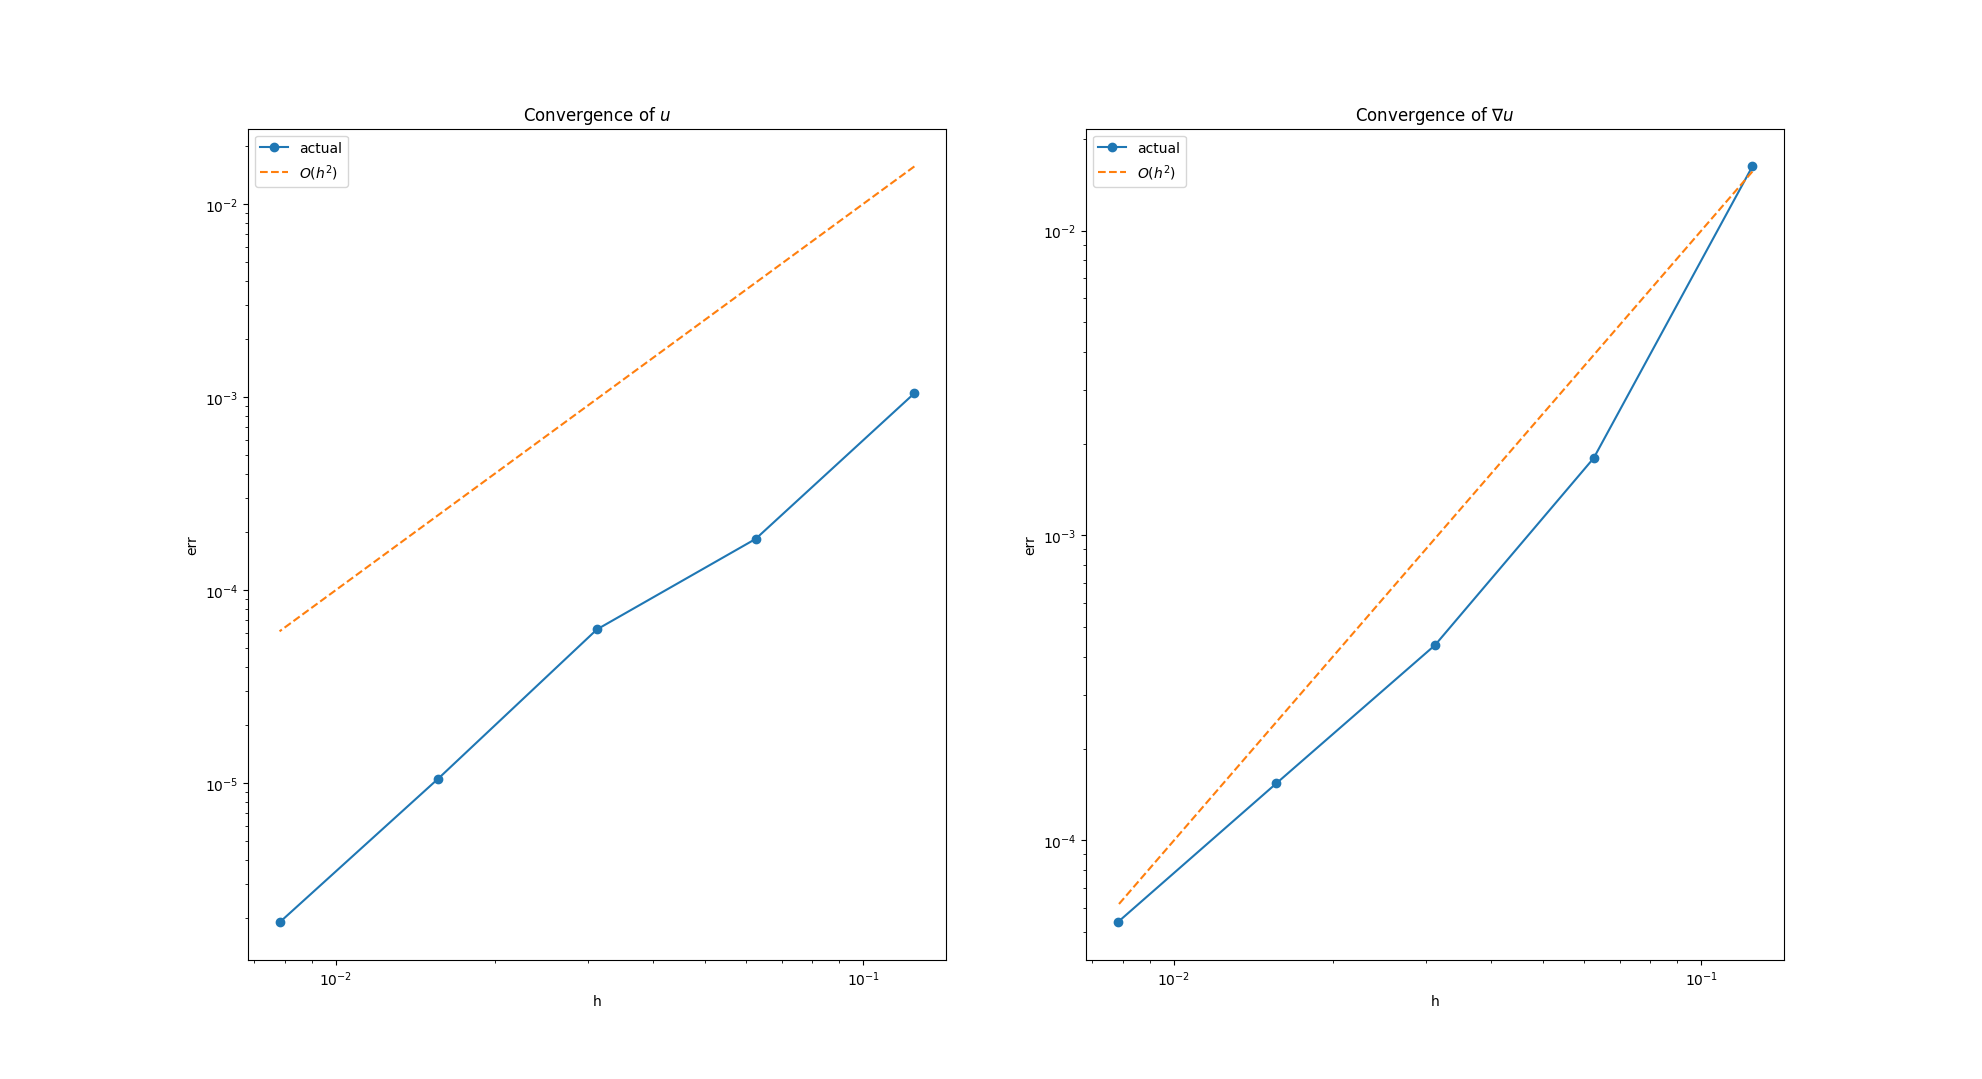
\includegraphics[width=0.95\textwidth]{figures/convergence_poisson.png}
	\caption{Convergence study for the Poisson equation with manufactured jump conditions.}
	\label{fig:poisson_convergence}
\end{figure}


\subsection{Test benchmarks}

After verifying the individual components (advection and Poisson), we now couple them and simulate two physically relevant problems.

\subsubsection{Plasma past a charged cylinder}

We consider a 2D2V Vlasov–Poisson system modelling a plasma flowing past a charged cylinder.  
The spatial domain is \((x,y)\in[0,L_x]\times[0,L_y]\), and the velocity domain is
\((v_x,v_y)\in[-5v_{th,i},\,15v_{th,i}]\times[-7v_{th,i},\,7v_{th,i}]\).  
The phase space is uniformly discretized with \((n_x,n_y,n_{v_x},n_{v_y}) = (160,50,120,50)\) interior cells and \(n_{\mathrm{gc}}=3\) ghost cells in each direction.  
The time step is \(\Delta t = 5\times10^{-4}\) and the final time is \(t_{\text{final}} = 0.15\).

Initially, no particles are present in the domain.  
Ions are injected through the left boundary via a shifted Maxwellian in \(v_x\) centred at \(v_x = 5v_{th,i}\).  
Zero inflow is imposed on the right boundary, and reflective conditions are used on the top and bottom boundaries.

Reference quantities are: \(x_0 = L_x\), \(m_0 = m_i\), \(n_0 = 1\;\text{m}^{-3}\), \(k_BT_0 = 0.15\;\text{eV}\).  
The charged cylinder is defined by \((x-0.375)^2 + y^2 = 0.125^2\).  
It is held at a potential \(\phi = -20\;\text{V}\); its permittivity is set to \(1000\) to mimic a conductor, while the surrounding vacuum has unity permittivity.  
The Poisson equation is solved with Dirichlet conditions on the inflow boundary (\(\phi=0\) at \(x=0\)) and homogeneous Neumann conditions elsewhere.

\begin{figure}[htbp!]
  \centering
  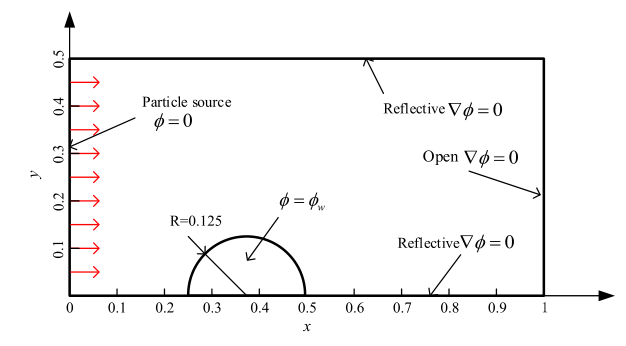
\includegraphics[width=0.7\textwidth]{figures/cylinder_setup.png}
  \caption{Schematic of the domain (normalised by \(L_x\)) and the boundary conditions.}
  \label{fig:cylinder_setup}
\end{figure}

\begin{figure}[htbp!]
	\centering
	\subfloat[Electric potential]{
		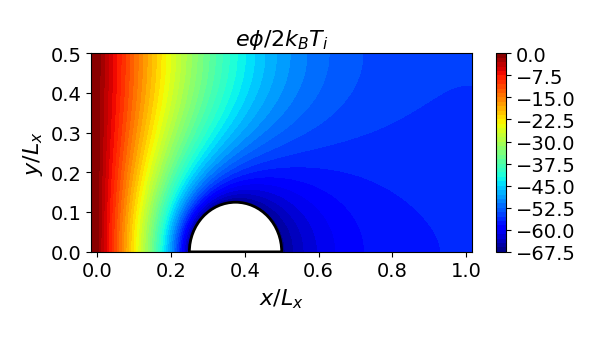
\includegraphics[width=0.5\textwidth]{figures/cylinder_potential.png}
	}
	\subfloat[Ion number density]{
		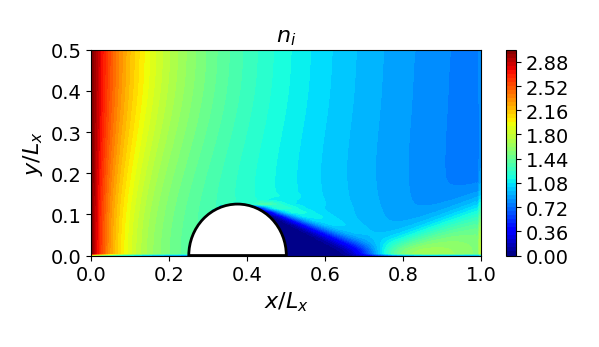
\includegraphics[width=0.5\textwidth]{figures/cylinder_number_density_ion.png}
	}
	\label{fig:cylinder}
\end{figure}

\subsubsection{Rough wall sheath problem}

Finally, we investigate the sheath formed near a wall with a rough surface.  
The spatial domain is \([0,20\lambda_D]^2\), where \(\lambda_D\) is the electron Debye length, discretised with \(n_x\times n_y = 100\times 50\).  
For electrons, the velocity space is \([-4v_{th,e},\,4v_{th,e}]\times[-5v_{th,e},\,5v_{th,e}]\) with \(v_{th,e}=\sqrt{k_BT_e/m_e}\); for ions, it is \([-4v_{th,i},\,4v_{th,i}]\times[-15v_{th,i},\,v_{th,i}]\) with \(v_{th,i}=\sqrt{k_BT_i/m_i}\).  
The time step is \(\Delta t = 0.015\) and the simulation runs for \(40\,000\) steps.  
Reference quantities are: \(L_0=\lambda_D\), \(m_0=m_e\), \(k_BT_0 = k_BT_e\), and \(T_i/T_e = 0.1\).

The wall consists of half‑circles, as shown in Fig.~\ref{fig:rough_wall_setup} (all dimensions are normalised by \(\lambda_D\)).  
On the wall, a Dirichlet condition \(\phi = -4\phi_0\) is imposed for the Poisson equation, and a zero‑inflow condition is used for the kinetic equations.

\begin{figure}[htbp!]
  \centering
  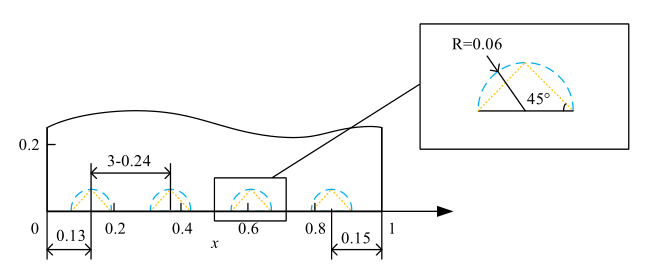
\includegraphics[width=0.7\textwidth]{figures/rough_wall_setup.png}
  \caption{Schematic of the rough wall domain (normalised by \(\lambda_D\)) and the boundary conditions.}
  \label{fig:rough_wall_setup}
\end{figure}

\begin{figure}[htbp!]
	\centering
	\subfloat[Electric potential]{
		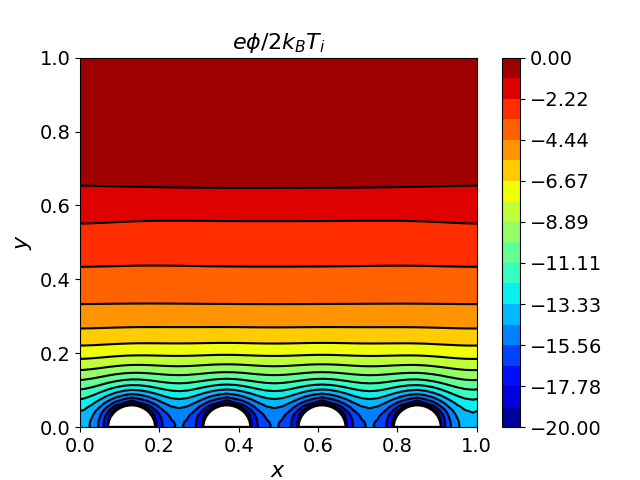
\includegraphics[width=0.5\textwidth]{figures/sheath_rough_wall_potential.png}
	}
	\subfloat[Electron number density]{
		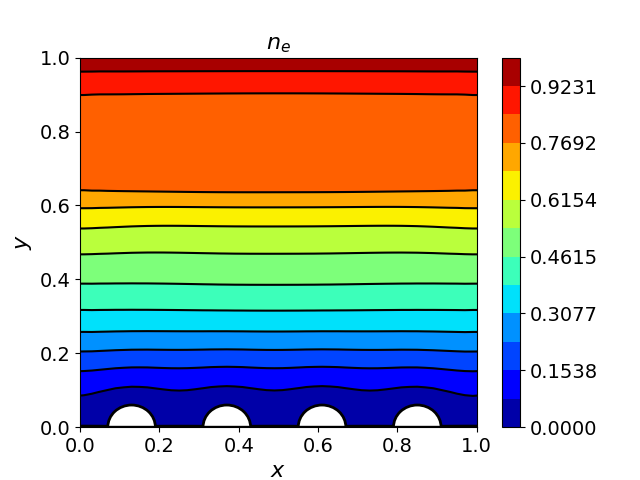
\includegraphics[width=0.5\textwidth]{figures/sheath_rough_wall_number_density_electron.png}
	}
	\label{fig:sheath_rough_wall}
\end{figure}